% ------------------------------------------------------------------------------
% TYPO3 CMS 8.3 - What's New (English Version)
%
% @author	Patrick Lobacher <patrick@lobacher.de> and Michael Schams <schams.net>
% @license	Creative Commons BY-NC-SA 3.0
% @link		http://typo3.org/download/release-notes/whats-new/
% @language	English
% ------------------------------------------------------------------------------
% LTXE-CHAPTER-UID:		07b25346-95b1df21-a6ebe09a-49f53f41
% LTXE-CHAPTER-NAME:	Backend User Interface
% ------------------------------------------------------------------------------

\section{Gebruikersinterface backend}
\begin{frame}[fragile]
	\frametitle{Gebruikersinterface backend}

	\begin{center}\huge{Hoofdstuk 1:}\end{center}
	\begin{center}\huge{\color{typo3darkgrey}\textbf{Gebruikersinterface backend}}\end{center}

\end{frame}

% ------------------------------------------------------------------------------
% LTXE-SLIDE-START
% LTXE-SLIDE-UID:		63dbe4be-21837dec-9bda98fe-ffad7ad7
% LTXE-SLIDE-ORIGIN:	a5b4032f-741b8eea-643674fb-4dc14f50 English
% LTXE-SLIDE-TITLE:		!Feature: #20446 - Clear cache entry in context menu
% LTXE-SLIDE-REFERENCE:	!Feature-20446-ClearCacheEntryInContextMenu.rst
% ------------------------------------------------------------------------------
\begin{frame}[fragile]
	\frametitle{Gebruikersinterface backend}
	\framesubtitle{"Clear Cache" optie in het contextmenu}

	Er is een nieuwe optie toegevoegd aan het contextmenu van de paginaboom. De optie is geplaatst in "Page actions"
	en maakt het mogelijk om de cache van de geselecteerde pagina te legen.

	\begin{figure}
		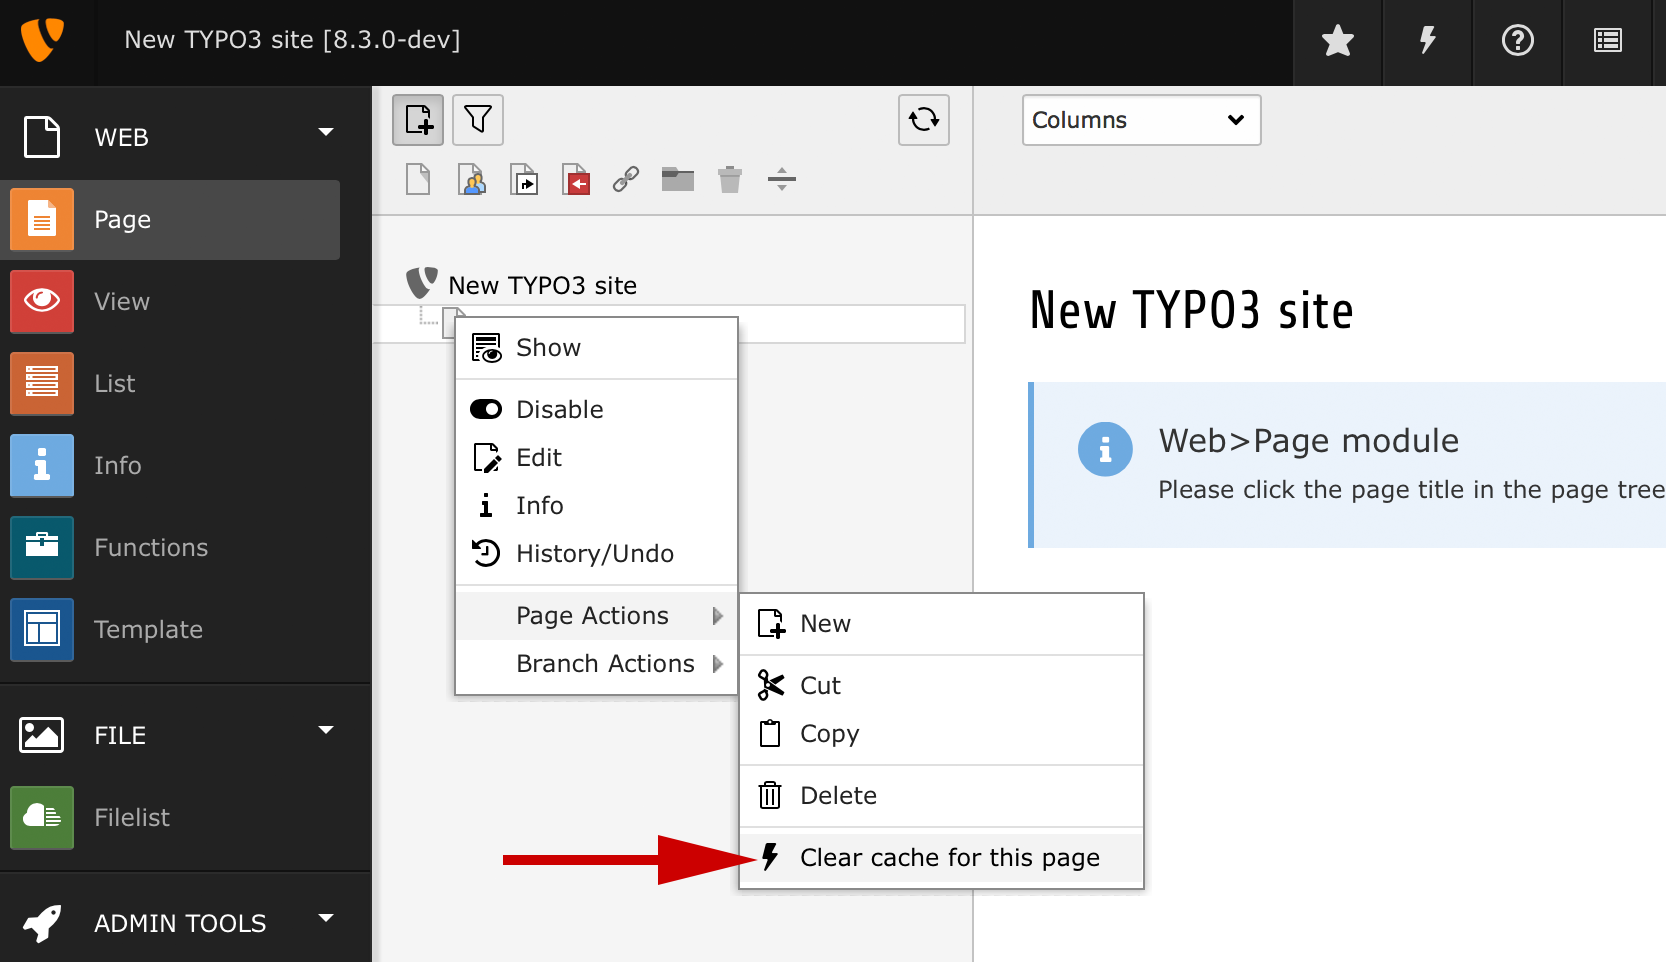
\includegraphics[width=0.70\linewidth]{BackendUserInterface/20446.png}
	\end{figure}

\end{frame}

% ------------------------------------------------------------------------------
% LTXE-SLIDE-START
% LTXE-SLIDE-UID:		e98c5d31-c3de5620-21a494fe-572fff60
% LTXE-SLIDE-ORIGIN:	5b0090eb-13043388-8c4dee34-6cac1521 English
% LTXE-SLIDE-TITLE:		!Feature: #76072 - Ogg, flac and opus support
% LTXE-SLIDE-REFERENCE:	!Feature-76072-OggFlacAndOpusSupport.rst
% ------------------------------------------------------------------------------
\begin{frame}[fragile]
	\frametitle{Gebruikersinterface backend}
	\framesubtitle{Ogg, Flac en Opus ondersteuning}

	Er is ondersteuning toegevoegd aan het media veld voor de volgende open formaten:
	\texttt{ogg}, \texttt{flac} en \texttt{opus}

	\begin{figure}
		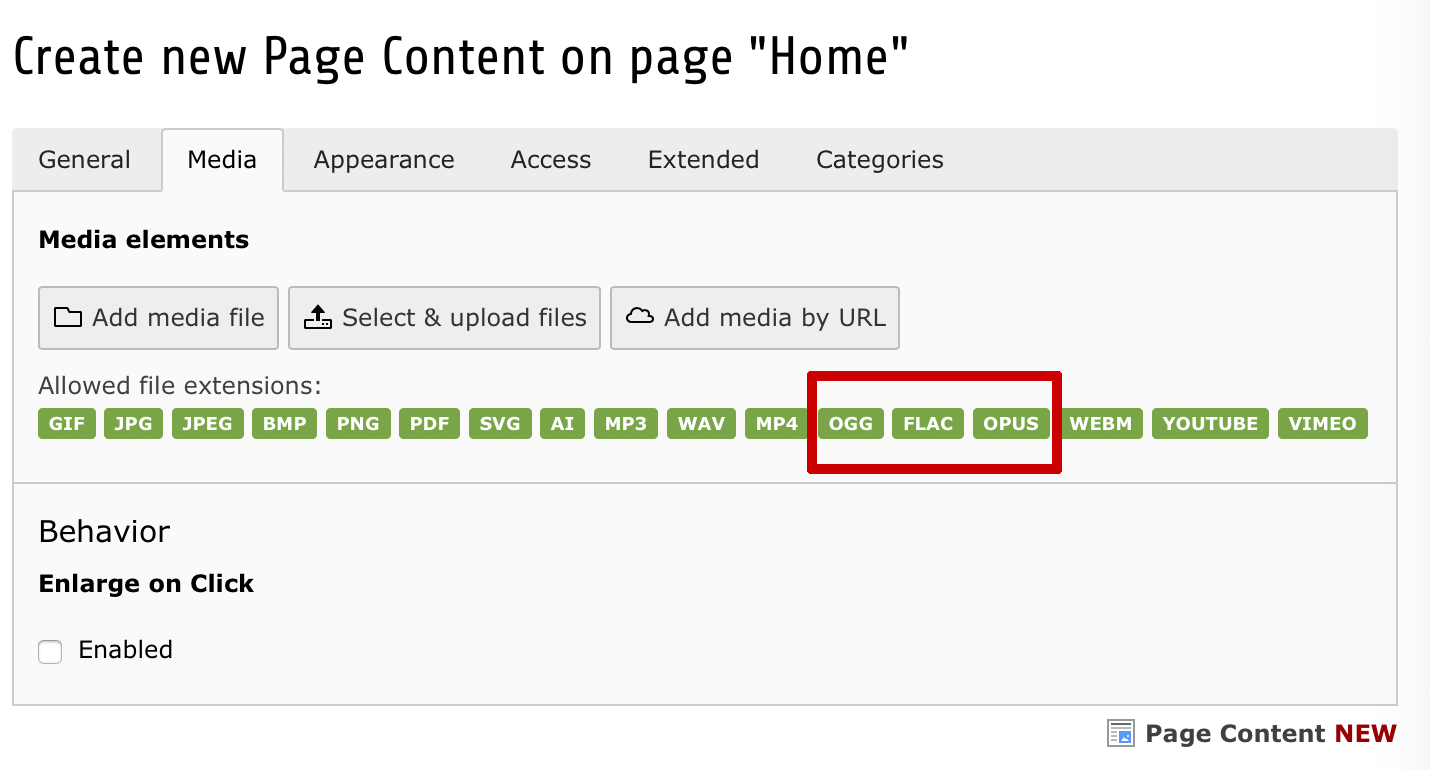
\includegraphics[width=0.70\linewidth]{BackendUserInterface/76072.png}
	\end{figure}

\end{frame}


